\chapter{AortaGeomRecon Research and Development}
This chapter will discuss about the research and development of the \progname{}. \\
AortaGeomRecon stands for Aorta Geometry Reconstruction. The main objective of this software is to semi-automatically build 3D geometry of the Aorta from the patient's chest ct scans.  The existing methods are often involved of extensive manual works with very complex software, with a minimum of 10 minutes of human operator, who are likely a medical domain expert. \\
The implementation till the date of this report can let the users who have the user characteristics described in SRS get the Aorta 3D geometry with only a few hyperparameters and 2 minutes of execution time. \\


\section{Existing Methods}
There are many segmentation software available to the users, we will discuss the two main methods on two softwares.


\begin{itemize}
\item ITK-Snap
ITK-Snap provides 
\item 3D Slicer
\end{itemize}

\section{3D Slicer Extension Development}

\section{Segmentation Algorithm}

This is a sample chapter

If you need to use quotes, type it ``like this''.

\section{GitHub and Workflows}

\section{Referencing}
These are some sample references to GAMYGDALA~\citep{popescu2014gamygdala} from 
the \texttt{references.bib} file and state effects of 
cognition~\citep{hudlicka2002time} from the \texttt{references\_another.bib} 
file. These references are not in the same .bib file.
%
%\section{Figures}
%This is a single image figure (Figure~\ref{fig_singleenv}):
%
%\begin{figure}[ht]
%    \centering
%    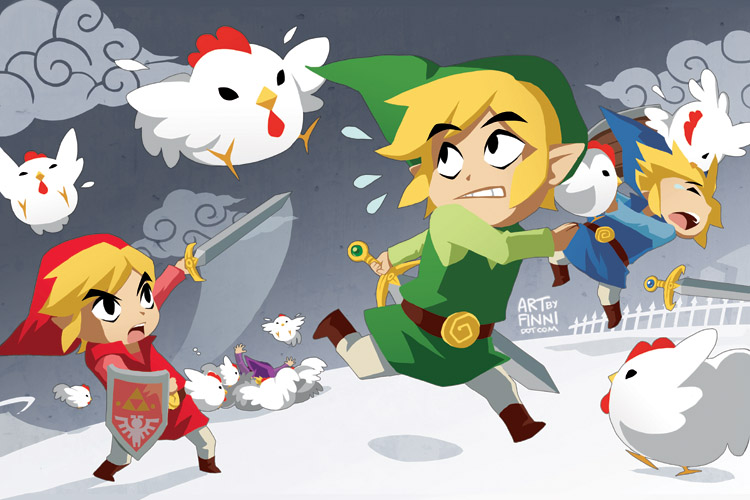
\includegraphics[width=0.6\textwidth]{figures/Sample/tumblr_static_eaceks0rfxsss8o4swscw40wo.jpg}
%    \caption[Single Figure Environment Listed Title]{This is a single figure 
%    environment}
%    \label{fig_singleenv}
%\end{figure}
%
%This is a multi-image figure with a top (Figure~\ref{fig_multienv_1}) and bottom (Figure~\ref{fig_multienv_2}) aligned subfigures:
%
%\begin{figure}[ht]
%	\centering
%	\begin{subfigure}[t]{\textwidth}
%		\centering
%		
%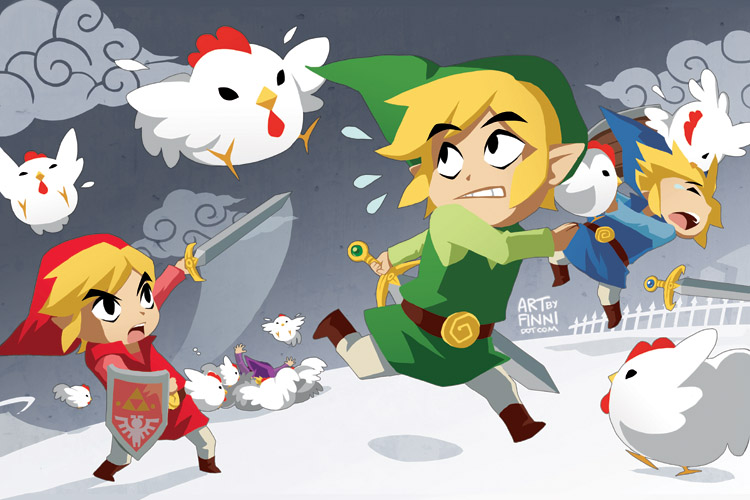
\includegraphics[width=0.7\textwidth]{figures/Sample/tumblr_static_eaceks0rfxsss8o4swscw40wo.jpg}
%		\caption{Figure 1}
%		\label{fig_multienv_1}
%	\end{subfigure}
%	~
%	\begin{subfigure}[t]{\textwidth}
%		\centering
%		
%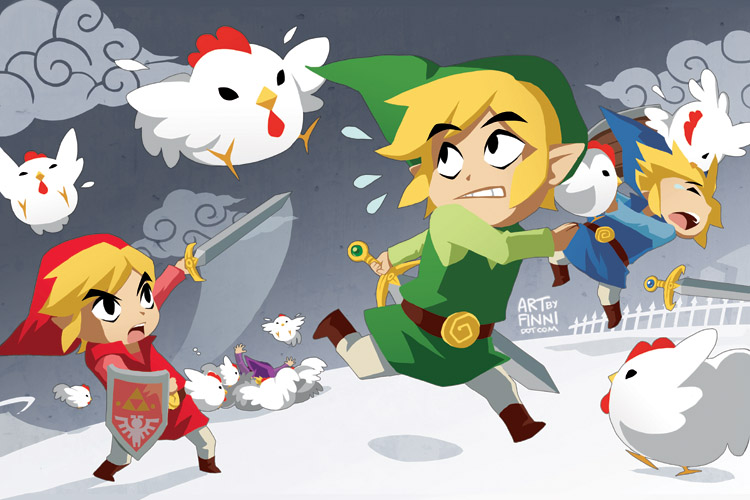
\includegraphics[width=0.7\textwidth]{figures/Sample/tumblr_static_eaceks0rfxsss8o4swscw40wo.jpg}
%		\caption{Figure 2}
%		\label{fig_multienv_2}
%	\end{subfigure}
%	
%	\caption{A Multi-Figure Environment}
%	\label{fig_multienv}
%\end{figure}
%
%\section{Tables}
%
%Here is a sample table (Table~\ref{tab_sample}):
%
%	\begin{table}[ht]
%	\centering
%	\begin{tabular}{ m{0.2\textwidth} m {0.1\textwidth} m{0.15\textwidth} }
%		\toprule
%		A & $\longleftrightarrow$ & B \\
%		C & $\longleftrightarrow$ & D \\
%		\bottomrule	
%	\end{tabular}	
%	\caption{A sample table}	
%	\label{tab_sample}
%\end{table}
%
%\subsection{Long Tables}
%A sample long table is shown in Appendix~\ref{appendix_b}.
%
%\section{Equations}
%
%Here is a sample equation (Equation~\ref{eq_lineslope}):
%
%\begin{equation} \label{eq_lineslope}
%	y = mx + b
%\end{equation}